\documentclass[tikz,dvipsnames]{standalone}
\usepackage[compat=1.1.0]{tikz-feynman}

\begin{document}

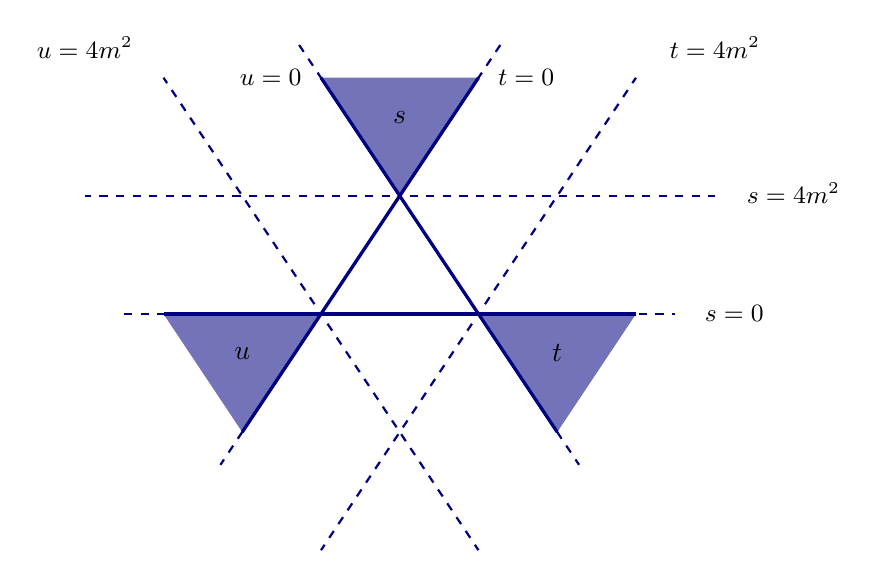
\begin{tikzpicture}[extended line/.style={shorten >=-#1,shorten <=-#1}]
		
    \node[label={[xshift=5cm, yshift=-0.35cm]\textcolor{Black}{\small{$s=4m^2$}}}] (a) at (0,0) {};
    \node[label=left:{\textcolor{Black}{\small{$u=0$}}}] (b) at (-1,1.5) {};
    \node[label=right:{\textcolor{Black}{\small{$t=0$}}}] (c) at (1,1.5) {};
    \node[label={[xshift=3cm]\textcolor{Black}{\small{$t=4m^2$}}}]  (m) at (1,1.5) {};
    \node[label={[xshift=-3cm]\textcolor{Black}{\small{$u=4m^2$}}}] (n) at (-1,1.5) {};
    \fill[NavyBlue!55] (a.center) -- (b.center) -- (c.center);


    \node (d) at (-1,-1.5) {};
    \node (e) at (-2,-3) {};
    \node (f) at (-3,-1.5) {};
    \fill[NavyBlue!55] (d.center) -- (e.center) -- (f.center);


    \node (g) at (1,-1.5) {};
    \node (h) at (2,-3) {};
    \node[label={[xshift=1.25cm, yshift=-0.35cm]\textcolor{Black}{\small{$s=0$}}}] (i) at (3,-1.5) {};
    \fill[NavyBlue!55] (g.center) -- (h.center) -- (i.center);


    \draw[extended line=0.5cm,thick,NavyBlue,dashed] (b.center) -- (h.center);
    
    \draw[extended line=0.5cm,thick,NavyBlue,dashed] (c.center) -- (e.center);
    \draw[very thick,NavyBlue] (c.center) -- (e.center);
    \draw[extended line=0.5cm,thick,NavyBlue,dashed] (f.center) -- (i.center);
    \draw[very thick,NavyBlue] (f.center) -- (i.center);
    \draw[very thick,NavyBlue] (b.center) -- (h.center);

    \draw[thick,NavyBlue,dashed] (a) -- +($(f)-(g)$);
    \draw[thick,NavyBlue,dashed] (a) -- +($(g)-(f)$);


    \draw[thick,NavyBlue,dashed] (d) -- +($(a)-(h)$);
    \draw[thick,NavyBlue,dashed] (d) -- +($(h)-(a)$);		

    \draw[thick,NavyBlue,dashed] (g) -- +($(a)-(e)$);
    \draw[thick,NavyBlue,dashed] (g) -- +($(e)-(a)$);
    
    \node (j) at (0,1) {\textcolor{Black}{$s$}};
    \node (k) at (-2,-2) {\textcolor{Black}{$u$}};
    \node (l) at (2,-2) {\textcolor{Black}{$t$}};

\end{tikzpicture}

\end{document}